% Лекции Сергея Борисовича Стечкина
% Внесены исправления Ю.Н.Субботина и Н.И.Черныха, версия 30.06.2009
% Внесены исправления Н.И.Черныха, версия 29.07.2009
% Внесена грамматическая и ТеХ-правка М.Дейкаловой, версия 05.08.09

\chapter{Интерполирование}   %%{Лекция 1.}

\section{Основные понятия}

\begin{defi}
{\it Метрическое пространство} $R=\{X,\ro\}$ -- это
множество $X$, между любыми двумя элементами $x,\, y$
которого определено расстояние $\ro(x,y)$, {удовлетворяющее
условиям}

1) $\ro(x,y)\ge 0,$ \ $\rho(x,y)=\rho(y,x)$\quad  $\forall \,x,y \in X;$

2) $\ro(x,y)=0 \Longleftrightarrow x=y;$

3) $\ro(x,y)\le \ro(x,z)+\ro(z,y)$\quad $\forall\, x,y,z \in X.$
\end{defi}

Пусть $\G M$~-- подмножество из $X,$\  $\G M \ne \varnothing,$\  $x \in X.$

\begin{defi}    %Определение
{\it Наилучшим приближением элемента $x$ элементами $\G M$} называется
величина
\[
{E(x)=}E(x,\G M)_R=\inf_{y \in \G M} \ro (x,y)=\ro (x,\G M) \ge 0.
\]
\end{defi}

{Для каждого элемента $x$ наряду} с $E(x,\G M)_R$
рассматривают множество $Y(x)$
наилучших элементов. {Итак,} $x \longmapsto Y(x) \subset X${:}
\[
  {y^* =} y^*{(x)} \in Y(x) \Longleftrightarrow  \begin{cases}
                            1) & y^* \in \G M,\\
                            2)  & \ro (x,y^*)=E(x,\G M)_R.
                           \end{cases}
\]

\begin{defi}
{Множество} $Y(x)$ называется множеством (многогранником)
наилучших элементов для $x$ или {\it множеством наилучших элементов
элемента} $x.$
\end{defi}

Может случиться, в частности, что {$Y(x)=\{y^*\}$} т.\,е. $y^*$~-- единственный
наилучший элемент для $x$ в $\G M.$ Так для $x \in \G M$ имеем $y^*=x,\ Y(x)=\{x\}.$

В следующем примере под кругом и далее под шаром в
любом нормированном пространстве понимаются соответствующие
замкнутые множества.

\begin{Example}
{Пусть $R=\{\bR^2, \ro\},$~ $\ro$ -- евклидово расстояние на плоскости
$\bR^2$,} $\G M$~-- круг {{(см. рис.~1.1)}} $x\notin \mathfrak{M},\
Y(x)=y^*$~-- одноэлементное множество. {Множество $Y(x)$} может быть пустым, например, если $\G
M$~-- внутренность круга, {и даже совпадать с $\G M$, например, если
$\G M$~-- окружность}, а ${x}$~-- ее центр.
\end{Example}

\begin{defi}
Если для любого элемента $x\in X,\ Y(x)\ne \varnothing,$ то
$\mathfrak{M}$ называется {\it множеством существования}, а
если $Y(x)$ -- одноточечное или пустое множество, то $\mathfrak{M}$
называется {\it множеством единственности.} В случае, когда
для любого $x\in X$ существует, причем единственный наилучший элемент в
$\mathfrak{M},$ то $\mathfrak{M}$ называется {\it чебышевским множеством.}
\end{defi}

%%%%%%%%%%%%%%%%%%%%%%%%%%%%%%%%%%%%%%%%%%%%%%%%%%%%%%
%\vspace{5mm}

\begin{figure}[ht]
\begin{center}
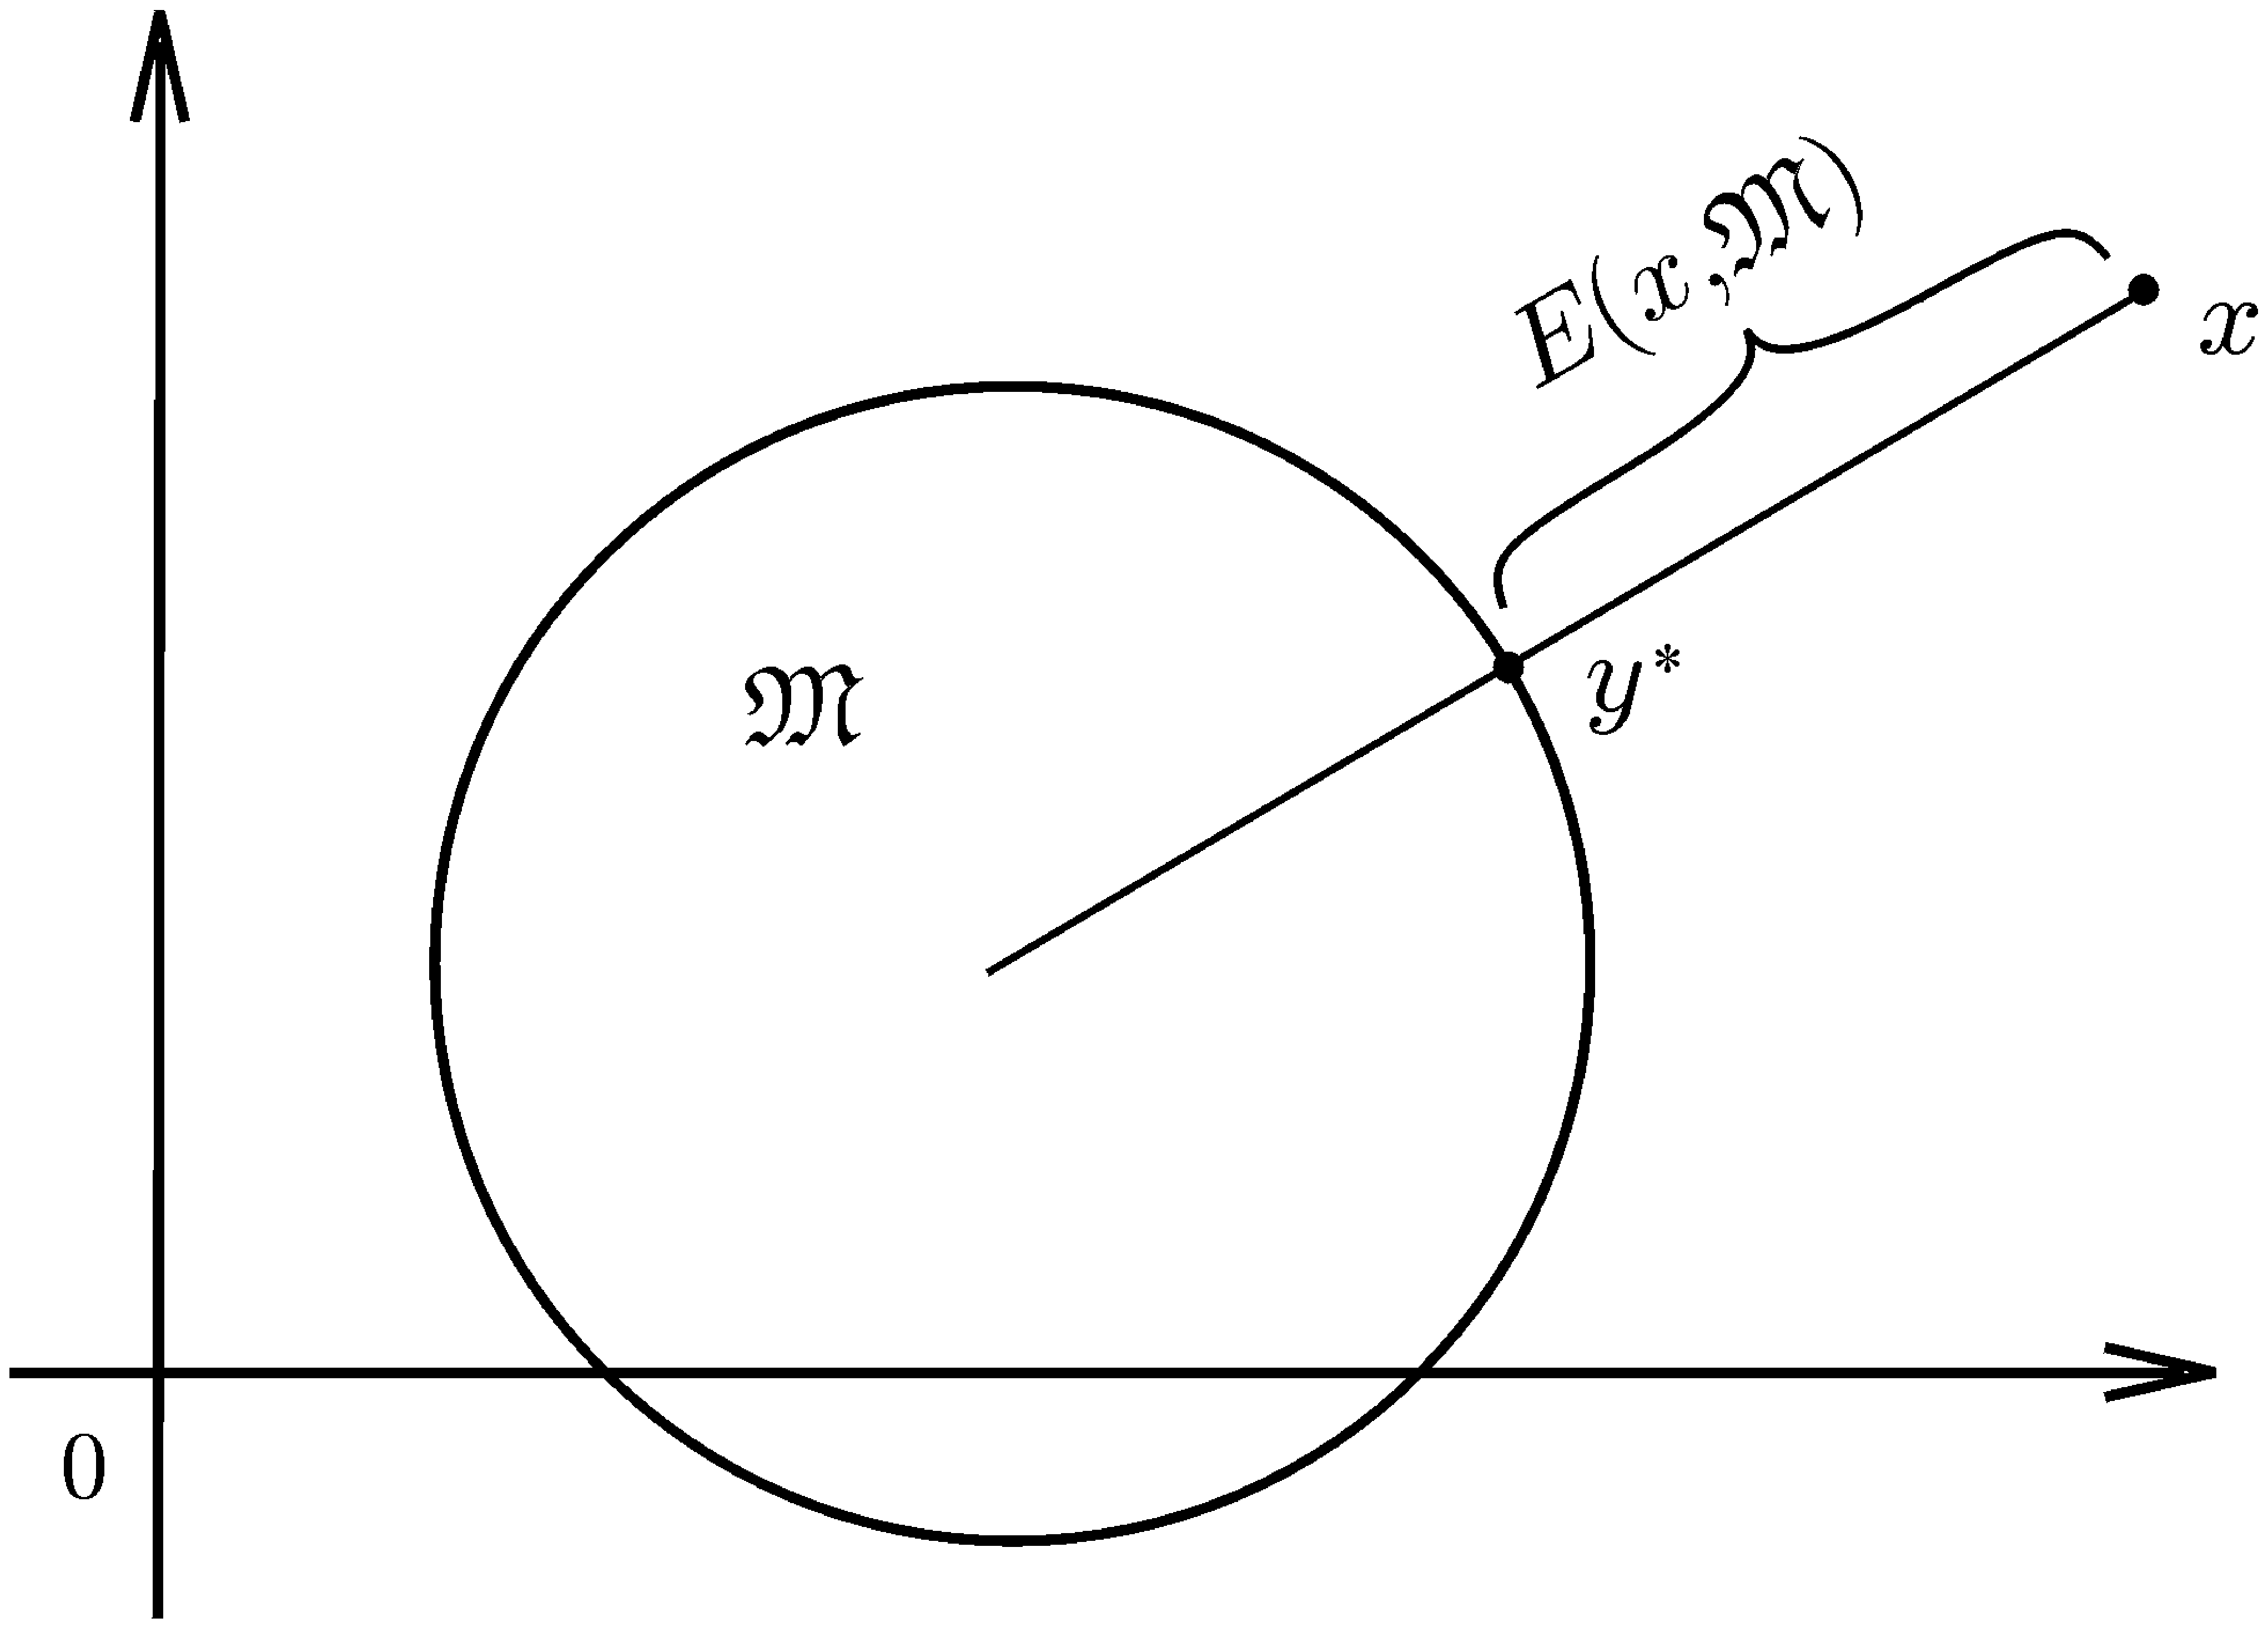
\includegraphics[width=0.5\textwidth]{pict01-1.eps}
\end{center}
 \bigskip
 \refstepcounter{ris}\label{r1-1}

 \centerline{Рис.~\theris}
 \bigskip
\end{figure}

% \bigskip
% \begin{picture}(70,170)
% \put(70,160){\special{em: graph pict1-1.eps}}
% \end{picture}
%\hbox to 0.5cm {}{\special{em:graph pict1.pcx}}
%\vspace{6cm}
% \bigskip
% \refstepcounter{ris}\label{r1-1}

% \centerline{Рис.~\theris}
% \bigskip

%%%%%%%%%%%%%%%%%%%%%%%%%%%%%%%%%%%%%%%%%%%%%%%%%%%%%%%%%%


Наилучшее приближение и наилучший элемент обладают и другими
неприятными особенностями. Поясним на
примере.

\begin{Example}
$X=C[a,b],$~ $-\infty < a < b < +\infty$ {(функция $f\in
C[a,b]$,} {если она непрерывна на $[a,b]$)},
{$\|f\|_C=\max\limits_{x\in[a,b]}|f(x)|$,}
$\ro(f,g)=\|f-g\|_C$. В качестве $\G M$ возьмем $\G M=\{c \}$
{--} множество констант $c \in \bR${, точнее, множество}
{постоянных функций}. Тогда, очевидно, {для любой} $ f
\in C[a,b]$ существует единственный наилучший элемент $c^* \in
\G M$, {
$$
c^* = \frac{\max\limits_{x\in[a,b]}{f(x)}+\min\limits_{x\in[a,b]} {f(x)}}{2}
$$
}
(см. рис.~\ref{r1-2}).
\end{Example}

%%%%%%%%%%%%%%%%%%%%%%%%%%%%%%%%%%%%%%%%%%%%%%%%%%%%%%
%\vspace{5mm}

\begin{figure}[ht]
\begin{center}
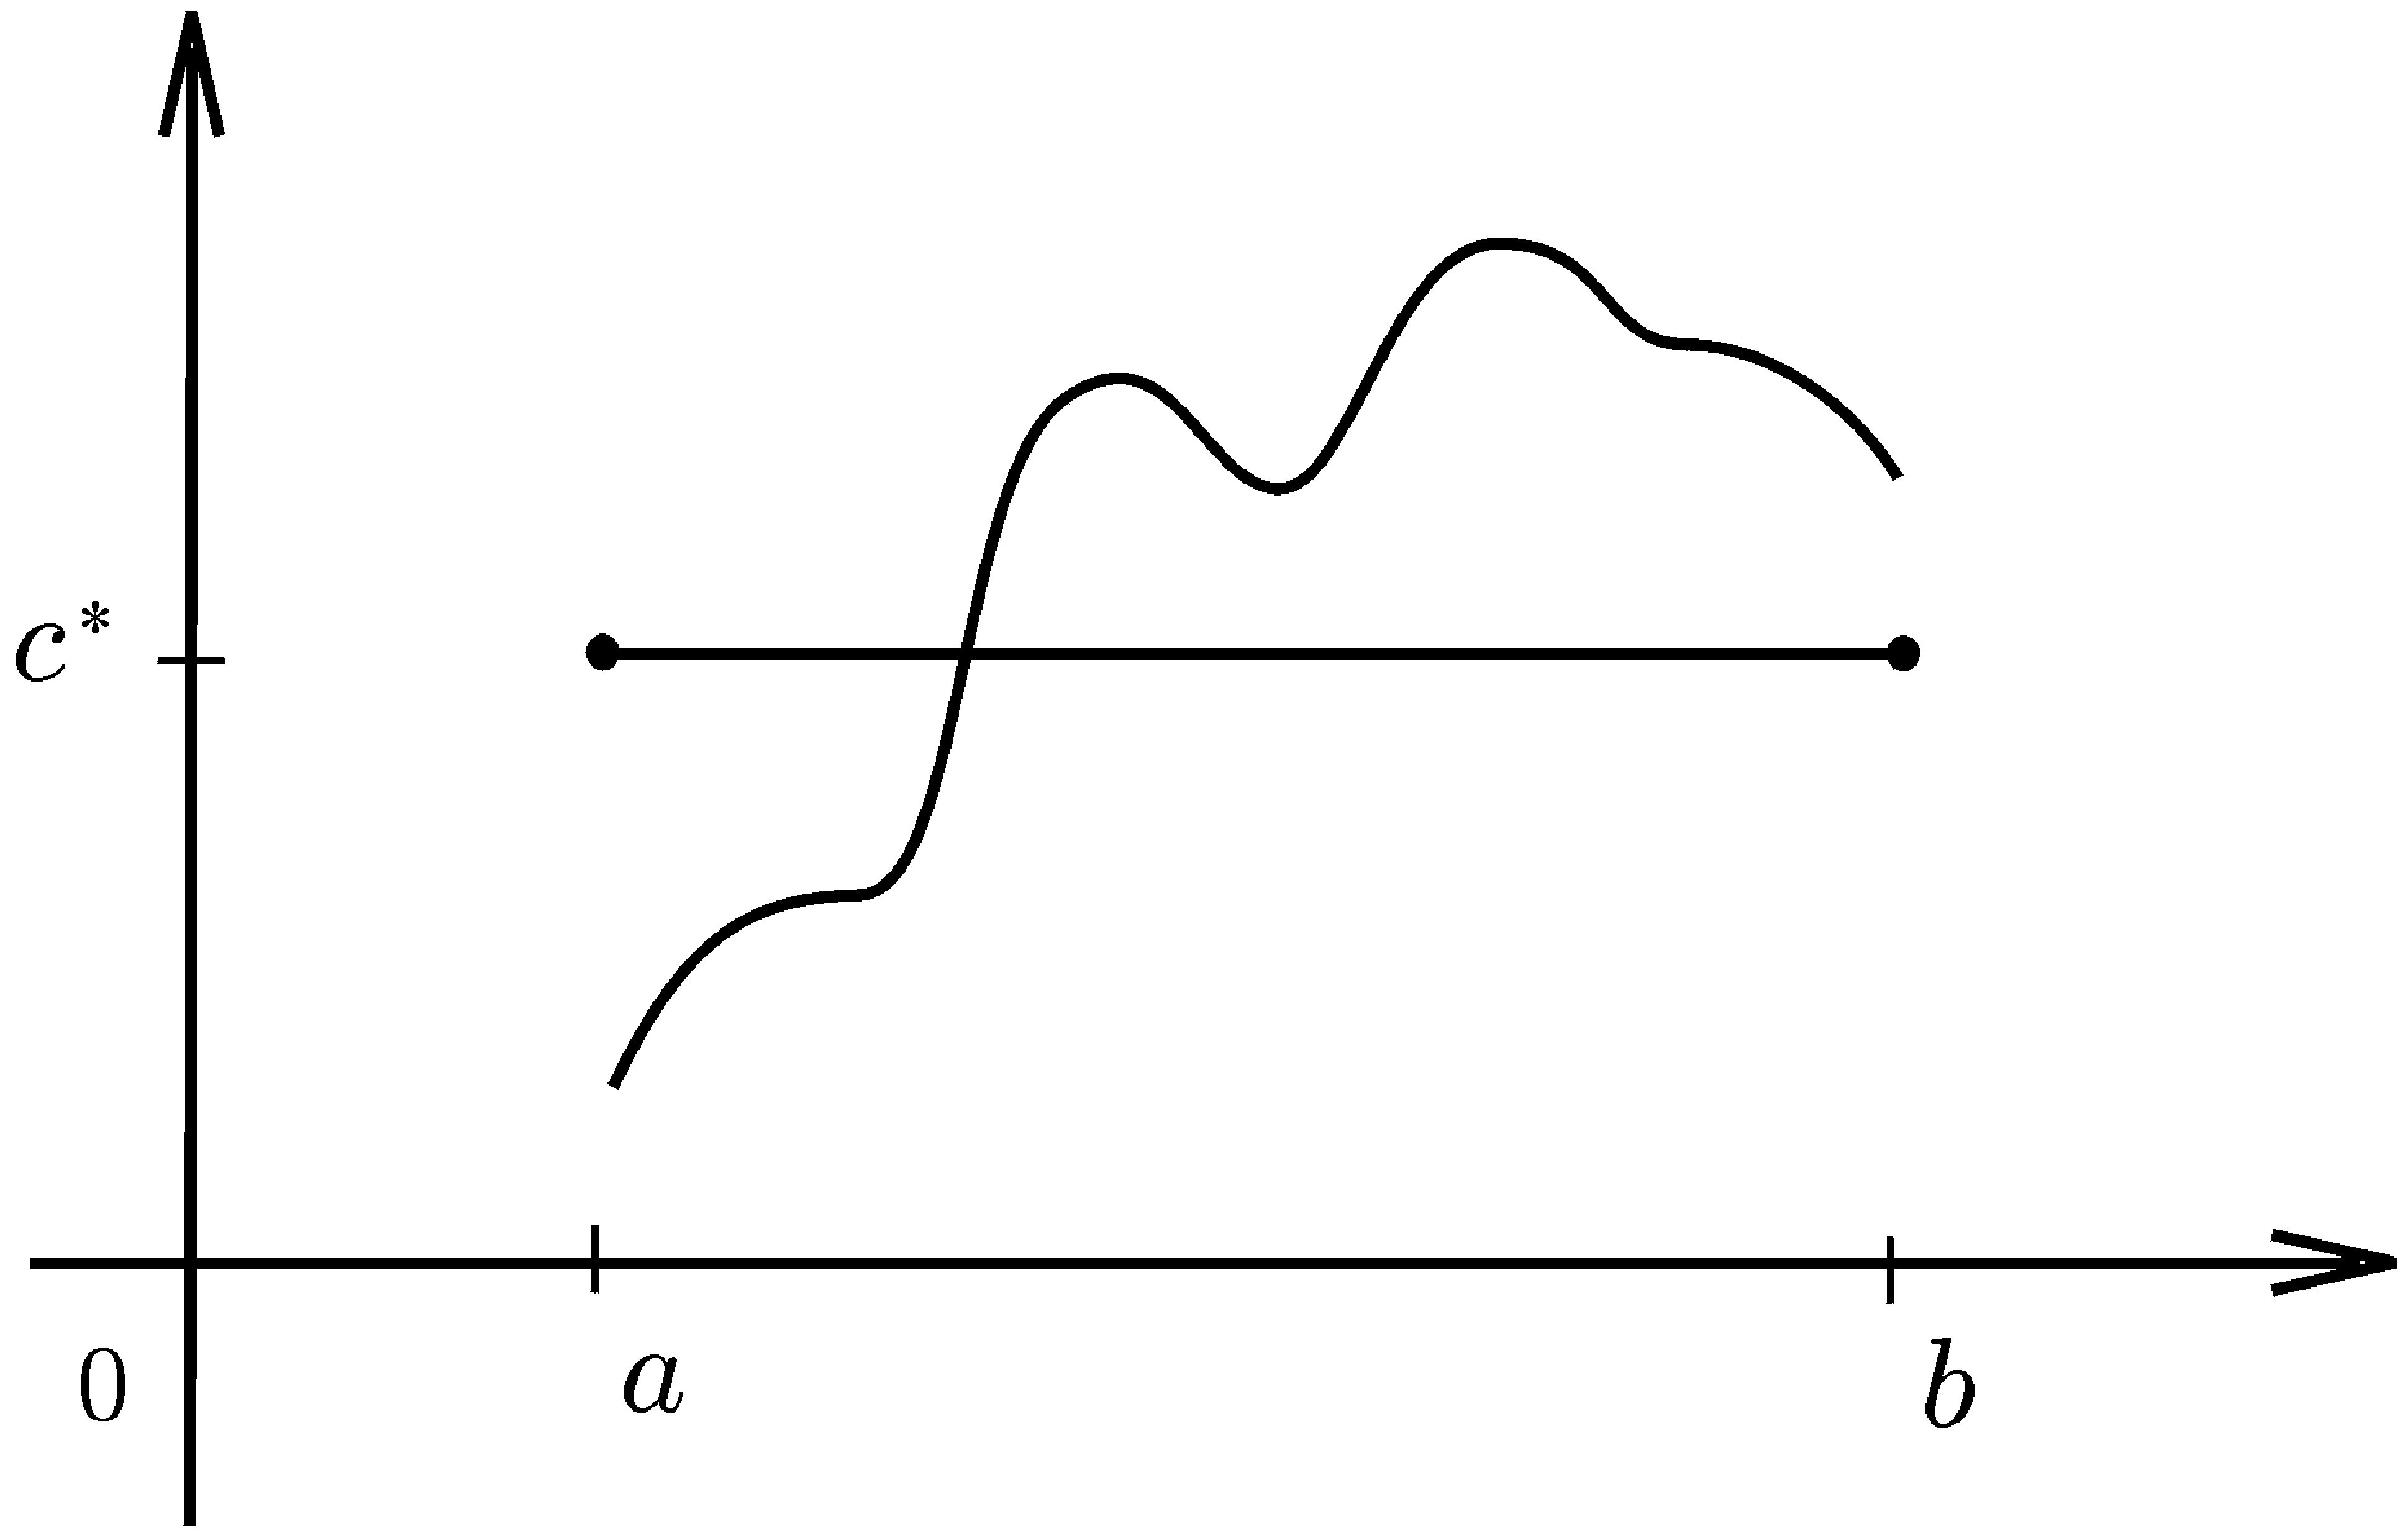
\includegraphics[width=0.5\textwidth]{pict01-2.eps}
\end{center}
 \bigskip
 \refstepcounter{ris}\label{r1-2}

 \centerline{Рис.~\theris}
 \bigskip
\end{figure}

% \bigskip
% \begin{picture}(70,170)
% \put(100,160){\special{em: graph pict01-2.eps}}
% \end{picture}
% \refstepcounter{ris}\label{r1-2}

% \centerline{Рис.~\theris}
% \bigskip

%%%%%%%%%%%%%%%%%%%%%%%%%%%%%%%%%%%%%%%%%%%%%%%%%%%%%%%%%%



Итак, возникает оператор {наилучшего приближения} $A${,}
любой функции $f \in C[a,b]$ ставящий в соответствие
наилучший элемент $c^* \in \G M$: $A(f)=c^*(f).$ Этот оператор не является линейным.
Действительно, если мы возьмем $f_1$ и $f_2$ как на рис.~\ref{r1-3}, то
$c^*(f_1)=c^*(f_2)=c^*(f_1+f_2)=h/2,$ т.\,е. $A(f_1+f_2)\ne A(f_1)+A(f_2).$

%%%%%%%%%%%%%%%%%%%%%%%%%%%%%%%%%%%%%%%%%%%%%%%%%%%%%%
%\vspace{5mm}

\begin{figure}[ht]
\begin{center}
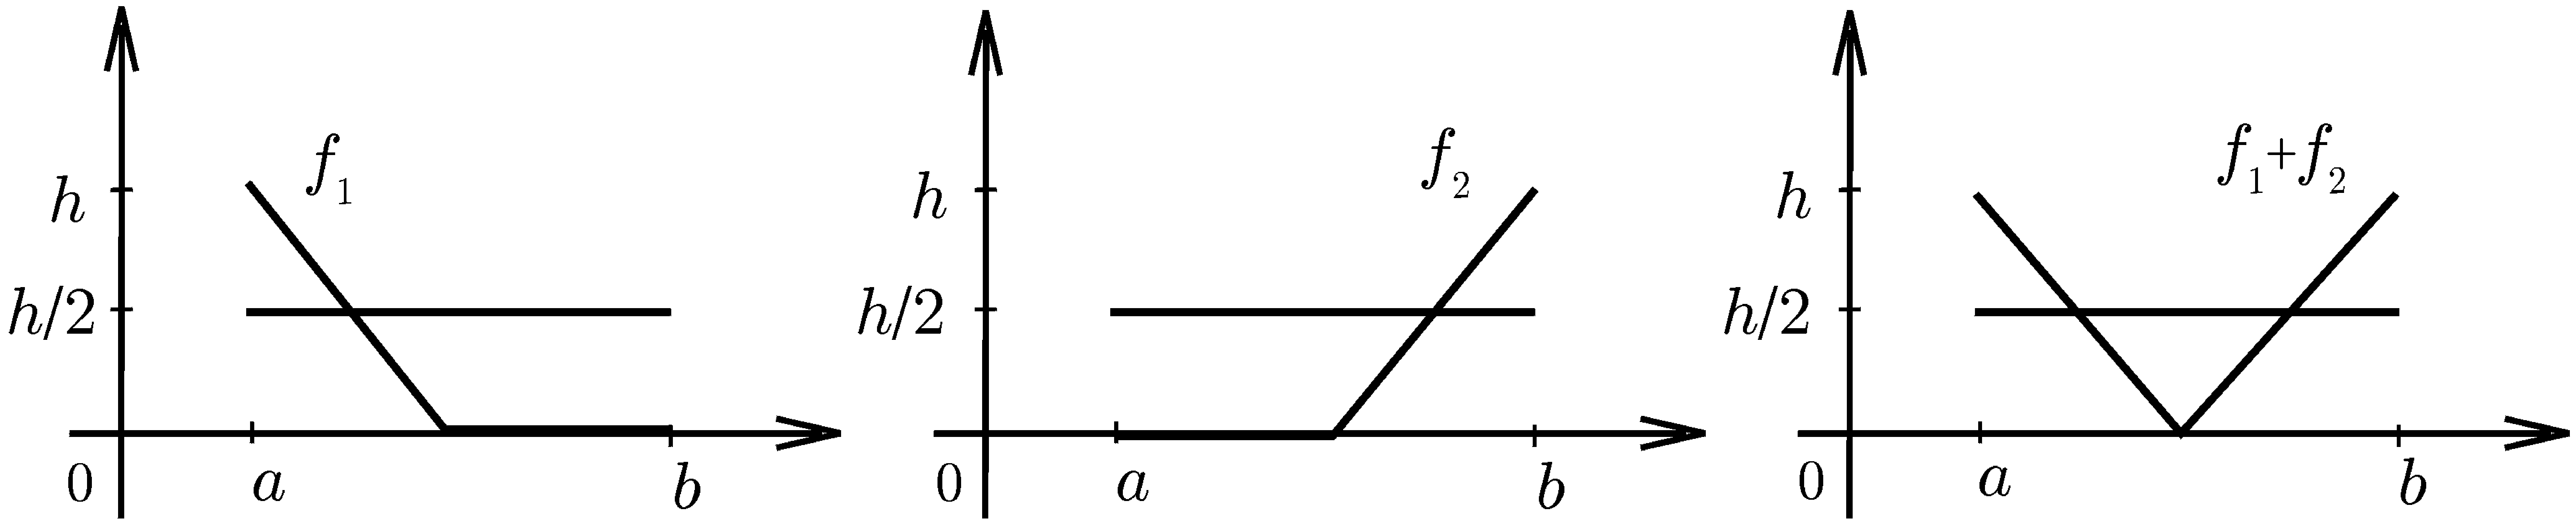
\includegraphics[width=0.9\textwidth]{pict01-3.eps}
\end{center}
 \bigskip
 \refstepcounter{ris}\label{r1-3}

 \centerline{Рис.~\theris}
 \bigskip
\end{figure}



% \bigskip
% \begin{picture}(0,120)
% \put(-10,120){\special{em: graph pict01-3.pcx}}
% \end{picture}
%\centerline{рис. 3} \vspace{5mm}
% \refstepcounter{ris}\label{r1-3}

% \centerline{Рис.~\theris}
% \bigskip

Итак, в некоторых функциональных пространствах {оператор наилучшего} {приближения}
$A$ не является линейным, значит,
{найти} $E{(x)}$ и $y^*{(x)}$ {может} {оказаться трудной задачей. Поэтому рассматривают и
более простые методы} {приближения. В частности, различные линейные методы.}

\section{Линейная задача теории приближения}

Пусть $X=C[a,b]=C$ и $\Cal L$ -- некоторое {подпространство} из $C$ и пусть $A$~--
линейный оператор из $C$ в $C$ и {$Af \in \Cal L$} для любой функции $f \in C[a,b].$
Будем говорить в этом случае, что в $C$ задан линейный метод $A$ приближения элементов
{из} $C$ посредством подпространства $\Cal L$. {Для $f$ в качестве приближающего
выступает элемент $Af$.}

Интерполирование -- первый классический метод линейного приближения.

\section{Лагранжево интерполирование}

Пусть функция $f \in C[a,b]$ (пока можно считать, что значения $f(x) \in \bC$~--
множеству комплексных чисел).

Возьмем на $[a,b]$ {различные точки} $x_k\ (k=0,1,\ldots,n)$. Можно считать, что
$a \le x_0 <x_1< \cdots <x_n \le b.$ Точки $\{x_k\}$ будут называться {\it узлами
интерполяции}.

Задача состоит в том, чтобы для узлов $\{x_k\}$ и для любого набора {чисел} $\{y_k\}\
(k=0,1,\dots ,n)$ построить многочлен $p_n \in \mathcal{P}_n,$
\[
  p_n(x)=a_0+a_1x+\cdots +a_n x^n,
\]
такой, что $p_n(x_k)=y_k$\  $(k=0,1,\dots ,n).$

Возникают вопросы:
\smallskip
1) Всегда ли задача разрешима?
\smallskip
2) Сколько имеется решений?
\smallskip

Здесь для определения коэффициентов $a_i\ (i=0,1,\dots,n)$ получается система линейных
уравнений с определителем Вандермонда, не равным $0.$ Следовательно, для любых $x_k$ и
любых $y_k$ имеется единственное решение. Поэтому достаточно {выписать} решение в
явном виде. {С этой целью для} любого $k=0,1,\dots,n$ построим фундаментальный
многочлен {$l_k(x)$} лагранжевой интерполяции, соответствующий $k$-му узлу, -- это
многочлен степени $n$, обладающий свойствами: $l_k(x_i)=\delta_{i,k}$, где
$\delta_{i,k}$ -- символ Кронекера, $\delta_{k,k}=1, \ \delta_{i,k}=0$ при $i \ne k$.

Очевидно,
\[
  l_k(x)=\frac{(x-x_0)(x-x_1)\cdots (x-x_{k-1})(x-x_{k+1})\cdots (x-x_n)}
         {(x_k-x_0)(x_k-x_1)\cdots (x_k-x_{k-1})(x_k-x_{k+1})\cdots (x_k-x_n)}.
\]
Обозначим $\omega(x)=\prod_{k=0}^n(x-x_k).$
Тогда
$$
\omega'(x_k)=
      (x_k-x_0)(x_k-x_1)\cdots (x_k-x_{k-1})(x_k-x_{k+1})\cdots (x_k-x_n)
$$
и, следовательно,
\[
 l_k(x)=\frac{\omega(x)}{(x-x_k)\omega'(x_k)}.
\]
Ясно, что
\[
 p_n(x)=p_{n}(x,\{y_k\},\{x_k\})=
 %\sum_{k=0}^n y_k
 %\frac{\omega(x)}{(x-x_k)\omega'(x_k)}=
 \sum\limits_{k=0}^n y_k l_k(x)
\]
-- искомый многочлен. Интерполяционный многочлен
рассматриваемой задачи, записанный в этой форме, называется {\it
интерполяционным многочленом Лагранжа}.

Пусть теперь $f \in C[a,b],$~ $\{x_k\}$~-- узлы интерполяции, а $y_k=f(x_k)$\
$(k=0,1,\dots ,n).$ Тогда для любой функции $f \in C[a,b]$ и любых узлов
{интерполяции} $\{x_k\}$\  $(k=0,1,\dots ,n)$ существует единственный многочлен
$$
p_n(x,f)=p_n(x,f,\{x_k\})=\sum\limits_{k=0}^n f(x_k) l_k(x)
$$
степени не выше $n$, который удовлетворяет условиям
\[
 p_n(x_k,f)=f(x_k)\qquad (k=0,1,\dots ,n).
\]
Таким образом, возникает {оператор} $P_n:\ f \longmapsto p_n(x,f)$ {из} $C{[a,
b]}$ в $C{[a,b]}$. {Отметим} простейшие свойства {этого оператора.}

1) {Если} $f \in \Cal P_n$, то для любых узлов $\{x_k\}$
имеем $p_n(x,f)\equiv f(x),$ т.\,е. $P_{n}(f)=f.$

2) $f \to P_n(\cdot,f)$
~-- линейный (т.\,е. однородный, аддитивный) ограниченный оператор:
$$
  P_n(c_1f_1+c_2f_2) \equiv c_1P_n(f_1)+c_2P_n(f_2),\qquad
  f_i\in C[a,b],\qquad c_i\in \bR\qquad (i=1,2),
$$
и для любой функции
$f\in C[a,b]$
$$
  \|p_n(\cdot,f)\|_C \le L_n\|f\|_C,\ \ \mbox{где}\ \
  L_n=\|P_n\|_C^C<\infty.
$$

Более того,
$$
|p_n(x,f)| \le L_n(x)\|f\|_C.
$$
Здесь $L_n(x)=\sum{|l_k(x)|},$~ $L_n =
\|L_n(x)\|_C$. Оба неравенства вытекают из формулы для $p_n(x, f) = p_n(x,f,\{x_k\})$. В
пространстве $C[a,b]$ они являются точными.

{Действительно, определим
при фиксированном $\xi \in [a,b]$ функцию $f_\xi(x)$ так,
чтобы она удовлетворяла условиям}

{а) $f_\xi(x)=\sign{l_k(\xi)}$ при $x=x_k\  ( k=0,1,\ldots,n)$,}

{б) $|f_\xi(x)| \le 1$ при $x \in [a,b]$,}

{в) $f_\xi(x)$ непрерывна по $x$ на $[a,b]$.}

{Тогда будем иметь
$$
\|f_\xi\|_C=1,
\qquad  p_n(x, f_\xi) = \sum\limits^n_{k=0}{f_\xi(x_k)l_k(x)}
$$
и, в частности,
$$
  p_n(\xi, f_\xi) = \sum\limits^n_{k=0}{|l_k(\xi)|} =
  L_n(\xi)\|f_\xi\|_C,
$$
а выбирая здесь в качестве $\xi$ точку $x^*$ максимума на $[a,b]$ функции $L_n(x)$,
получим
$$
  p_n(x^*,f_{x^*}(\cdot)) = L_n\|f_{x^*}\|_C
$$
и, следовательно,
$$
  \|p_n(x,f_{x^*}(\cdot))\|_C = L_n\|f_{x^*}\|_C.
$$}

{Таким образом, константа $L_n$ есть норма оператора $P_n\colon f \longmapsto p_n(x,f):$
$$
  \|P_n\|_{C \to C} = L_n.
$$
А для любого фиксированного $x \in [a,b]$ величина $L_n(x)$ является нормой функционала
$P_x(f)=p_n(x,f)$ в $C[a,b]$:
$$
\|P_x(f)\| = L_n(x),
$$
так как
$$
|P_x(f)| \le L_n(x)\|f\|_C\qquad \forall\ f \in C[a,b]
$$
и
$$
|P_x(f_x(\cdot))|=L_n(x)\|f_x\|_C.
$$}

{Константа $L_n$ называется \textit{константой Лебега}, а $L_n(x)$ --
\textit{функцией Лебега} линейного метода $p_n(x, f, \{x_k\})$ приближения функций $f$ из
$C[a,b]$ интерполяционными многочленами Лагранжа. Ясно, как эти понятия распространяются
на другие линейные методы приближения.}

{Метод интерполирования тем <<лучше>>, чем меньше его норма, т.\,е. константа Лебега. При
$n$ фиксированном $L_n$ зависит от узлов интерполирования $\{x_k\}$. Если $[a,b]=[-1,1]$,
то можно узлы выбрать так, что $L_n=\dfrac{2}{\pi}\ln{n} + O(1)$~ $(n \to +\infty)$, а
именно, в качестве узлов интерполяции нужно взять нули многочлена Чебышева
$$
T_{n+1}(x)=\cos({(n+1)}\arccos{x}).
$$}

3) Тождества Коши.

Из свойства 1) и формулы для интерполяционного многочлена {при $f(x)\equiv 1$}
получаем {тождество}
\[ \sum\limits_{k=0}^n l_k(x) \equiv 1, \]
{а при} $f(x)=(x-u)^j$~ $(j=1,\dots ,n;\ u\in \mathbb C)$ {-- тождества}
$$
(x-u)^j\equiv \sum\limits_{k=0}^n (x_k-u)^j l_k(x) \qquad (j=1,2,\ldots,n),
$$
{откуда при} $u=x$ следует, {что}
\begin{equation}\label{f1-1}
\sum\limits_{k=0}^n (x_k-x)^j l_k(x)\equiv 0\qquad (j=1,\ldots ,n).
\end{equation}
Эти тождества при $\{x_n\}\subset [a,b]$ справедливы для
всех $x\in \mathbb C.$

\section{Оценка погрешности интерполяционной \\ формулы
Лагранжа. Неравенства Лебега}

Пусть $\{x_k\}_{k=0}^n$~-- узлы интерполяции, $f \in C[a,b],$ $p_n(x,f)$ --
соответствующий интерполяционный многочлен Лагранжа. Можно написать
\[
  f(x)=p_n(x,f)+R_n(x,f),
\]
где $R_n(x,f)$~-- остаточный член. Очевидно, в узлах интерполяции $R_n(x_k,f)=0$~
$(k=0,\dots ,n).$ Требуется оценить $R_n(x,f)$ для любого фиксированного $x \in [a,b],$
а также оценить $\|R_n(\cdot ,f)\|_{C[a,b]}.$

Оказывается, для оценок остаточного члена лагранжевой интерполяции {достаточно} знать
$L_n(x),$ $L_n$ {и} $E(f ,\Cal P_n)_C=\inf\limits_{q \in \Cal P_n}\|f-q\|_{{C}}.$
Именно, имеют место неравенства Лебега
\[  |R_n(x,f)|\le (L_n(x)+1)E(f ,\Cal P_n)_C,             \]
\[  \|R_n(\cdot ,f)\|_{{C}} \le (L_n+1)E(f ,\Cal P_n)_C.             \]
Для доказательства воспользуемся тем, что $P_n(x,f)$~-- линейный оператор, и
$P_n(x,q)=q(x)$ для любого $q \in \Cal P_n$ ({аналогичные неравенства} Лебега
{возникают} и {для} более {общих линейных методов, сохраняющих элементы $\Cal
P_n$ на месте}). Имеем
\begin{multline*}
  |R_n(x,f)|=|f(x)-p_n(x,f)|=|f(x)-q(x)-p_n(x,f-q)|\le  \\
  \le |f(x)-q(x)|+L_n(x)\|f-q\| \le
      (L_n(x)+1)\|f-q\|_{{C}}, \qquad q \in \Cal P_n.
\end{multline*}
Значит, если в качестве $q$
возьмем наилучший элемент для $f$
в $\Cal P_n,$
то получим
\[  |R_n(x,f)|\le (L_n(x)+1)E(f ,\Cal P_n)_C,\qquad x\in [a,b],   \]
откуда следует, что
\[  \|R_n(\cdot ,f)\|_{{C}} \le (L_n+1)E(f ,\Cal P_n)_C.             \]

\section{Остаточный член в форме Коши\\
 для интерполяционной формулы Лагранжа}

%%%%%%%%%%%%%%%%%%%%%%%%%%%%%%%%%%%%%%%%%%%%%%%%%%%%%%%%%
{Функция $f \in C^{(n+1)}[a,b],$ если $f$ непрерывна на $[a,b]$ вместе с производными
до} {порядка $n+1$ включительно.}

\begin{teo}\label{t1-1}
Пусть $f \in C^{(n+1)}[a,b].$ Тогда для любого $x \in [a,b]$ существует {точка} $\xi
\in (a,b)$ {такая}, что
\[
  R_n(x,f)=\frac{f^{(n+1)}(\xi)}{(n+1)!}\omega (x)
\]
$(${здесь $\xi=\xi(x,f,\{x_k\})$},~ $n+1$~-- число узлов
интерполяции$).$
\end{teo}

\begin{proof}
{Доказываемая формула, очевидно, верна для $x=x_k$}
{$(k=0,\dots ,n)$} ($\xi$ может любой точкой). Зафиксируем {$x \in [a,b],$~ $x \ne x_k,$}
и рассмотрим вспомогательную функцию
\[
  F(t)=f(t)-p_n(t)-K\omega (t),
\]
где {$p_n(t)=p_n(t,f,\{x_k\}),$~ $K=R_n(x,f)/ \omega (x), \ \omega(x) \ne 0.$} Заметим,
что $F(t)$ при $t=x_k$ равна нулю $(k=0,\dots ,n)$ и $F(x)=0$ по выбору $K.$ Следовательно, функция
{$F(t)$} имеет нули в ${n+2}$ различных точках. Применим обобщенную теорему Ролля, из
которой следует, что найдется точка $\xi \in (a,b)$ такая, что $F^{(n+1)}(\xi)=0$.
{Но} $F^{(n+1)}(\xi)=f^{(n+1)}(\xi)-K\cdot (n+1)!,$ значит,
$K=f^{(n+1)}(\xi)/(n+1)!,$ откуда {для} $R_n(x,f)=K\omega(x)$ {получаем}
\[
  R_n(x,f)=\frac{f^{(n+1)}(\xi)}{(n+1)!}\omega (x)
\]
и теорема доказана.
\end{proof}

\begin{Remark}[геометрическое]
{Остаточный} член не обязан менять знак в узлах {интерполяции вслед за
$\omega(x).$} Графики $f(x)$ и $p_n(x,f)$ могут соприкасаться, как показано на
рис.~\ref{r1-4}.
\end{Remark}

%%%%%%%%%%%%%%%%%%%%%%%%%%%%%%%%%%%%%%%%%%%%%%%%%%%%%%
%\vspace{5mm}

\begin{figure}[ht]
\begin{center}
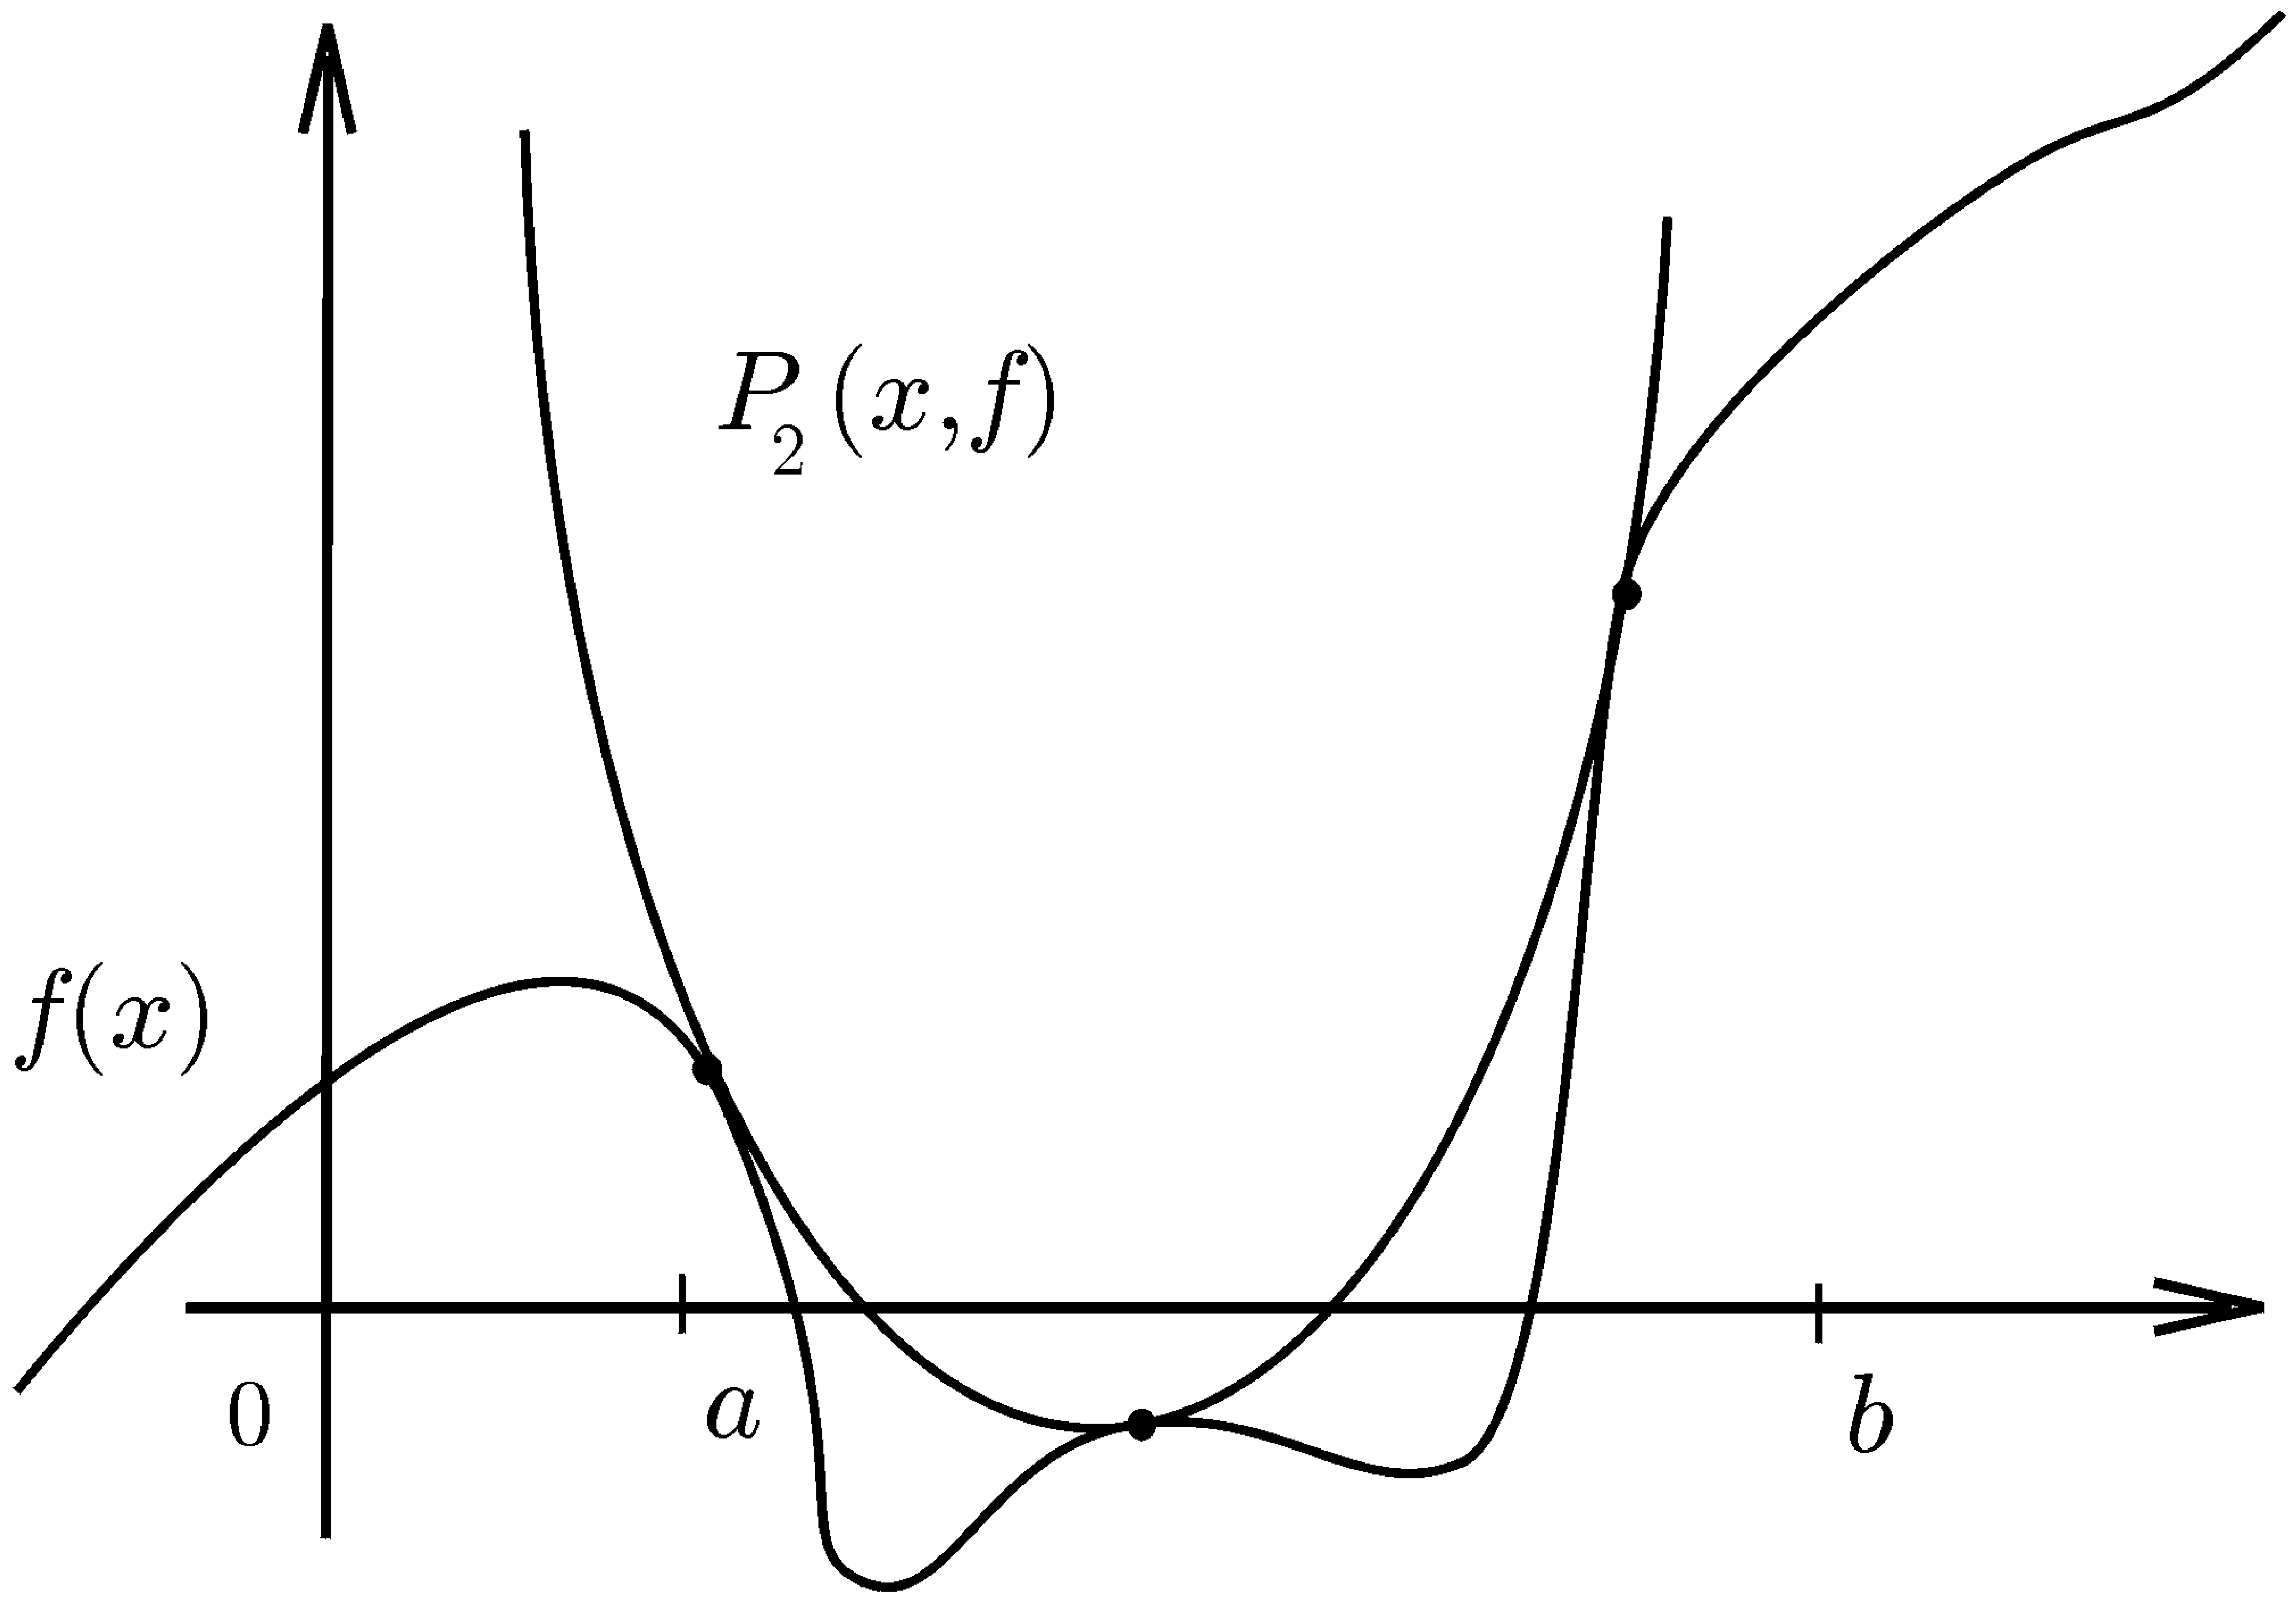
\includegraphics[width=0.5\textwidth]{pict01-4.eps}
\end{center}
 \bigskip
 \refstepcounter{ris}\label{r1-4}

 \centerline{Рис.~\theris}
 \bigskip
\end{figure}



% \bigskip
% \begin{picture}(70,190)
% \put(90,190){\special{em: graph pict01-4.pcx}}
% \end{picture}
%\hbox to 0.5cm {}{\special{em:graph pict4.pcx}}
%\vspace{6cm}

% \refstepcounter{ris}\label{r1-4}

% \centerline{Рис.~\theris}
% \bigskip

%%%%%%%%%%%%%%%%%%%%%%%%%%%%%%%%%%%%%%%%%%%%%%%%%%%%%%%%%%
%\noindent \hskip3.0cm {\rm рис. 4}
%\bigskip



Но есть достаточное условие того, что остаточный член меняет знак в узлах. Как видно из
формулы для остаточного члена интерполяции в форме Коши, {\it если} $f^{(n+1)}(x)$
{\it сохраняет знак}, {\it то} $R_n(x,f)$ {\it меняет знак в узлах интерполяции и только в них}.

Обозначим $M_{n+1}(f)=\max\limits_{x \in [a,b]}f^{(n+1)}(x).$

\begin{Corollary}
\[
 \|R_n(\cdot ,f) \|_C \le \frac{M_{n+1}(f)}{(n+1)!}\|\omega(\cdot ) \|_C .
\]
\end{Corollary}

\begin{task}
При каком выборе узлов интерполяции величина $\|\omega(\cdot ) \|_C$
наименьшая?
\end{task}

 Оказывается {это будет,} когда $\omega$~-- многочлен
Чебышева\footnote{{Свойства} многочлена Чебышева приводятся в лекции 2.}
{$\widetilde{T}_{n+1}(x,I)$ $(I=[a,b]).$}
{Действительно, } $\omega(x)=x^{n+1} +a_{n}x^n+ \dots +a_0.$ Так {что}
\[
  \inf \|\omega(\cdot)\|_{C[a,b]}=\|\widetilde{T}_{n+1}(\cdot{, I})\|_{C[a,b]},
\]
где $\widetilde{T}_{n+1}{(\cdot, I)}$~-- многочлен Чебышева
на $[a,b],$ т.\,е. наименее
уклоняющийся на $[a,b]$ от нуля многочлен {степени $n+1$} со
старшим коэффициентом 1. В частности, $\widetilde{T}_{n+1}(x,[-1,1])=
\dfrac1{2^n}\cos(n+1)\arccos x.$


\section{Теорема Хаара об интерполяции в $\mathbb R^N$}

Мы рассматривали {задачу} интерполяции на {$D=[a,b] \subset
\bR^1$} т.\,е. в одномерном случае. Пусть теперь множество {$D \subset \bR^N,\ N\ge 2.$}

{{В о п р о с ы}. \hspace{1em}}

Имеет ли смысл задача {интерполяции} в многомерном случае?

Существуют ли действительные функции {$f_0(x),f_1(x),\dots,f_n(x),$~ $x \in
\overline{D} \subset \bR^N,$} ({\it интерполяционные системы на} $D$), {линейными
комбинациями которых} можно интерполировать {любой набор чисел $\{y_k\}_{k=0}^n$ в} любых
{несовпадающих узлах} $\{x_k\}_{k=0}^n \in D?$

Легко убедиться, что интерполяционные системы, состоящие из
разрывных функций, существуют на любом множестве мощности континуум. Для
этого достаточно рассмотреть взаимно однозначное
отображение отрезка на множество и взять порожденные им функции,
соответствующие рассмотренной нами на отрезке
интерполяционной системе $1,x,x^2,\dots ,x^n.$

Далее будет показано, что задача интерполяции многочленами разрешима
в комплексной области. А ответ на вопрос об $\bR^N$ дает следующая теорема.

\begin{teo}[А.\,Хаар]
Если $N>1$ и множество $D\subset \mathbb R^N$ имеет
внутренние точки, т.\,е. {$\inter {D} \ne \varnothing,$} и если $n \ne 0,$ то {в
$D$ не существует} непрерывных действительных интерполяционных систем {$($т.\,е.
систем, которыми можно интерполировать} при любом выборе узлов $\{x_k\}^{n}_{k=0}$
любой набор чисел $\{ y_k\}_{k=0}^n).$
\end{teo}

\begin{proof}
Возьмем внутреннюю точку и ее некоторую
окрестность $\Delta \subset D,$
и пусть {$\{x_k\}_{k=0}^n \subset \Delta.$}

%%%%%%%%%%%%%%%%%%%%%%%%%%%%%%%%%%%%%%%%%%%%%%%%%%%%%%

\begin{figure}[ht]
\begin{center}
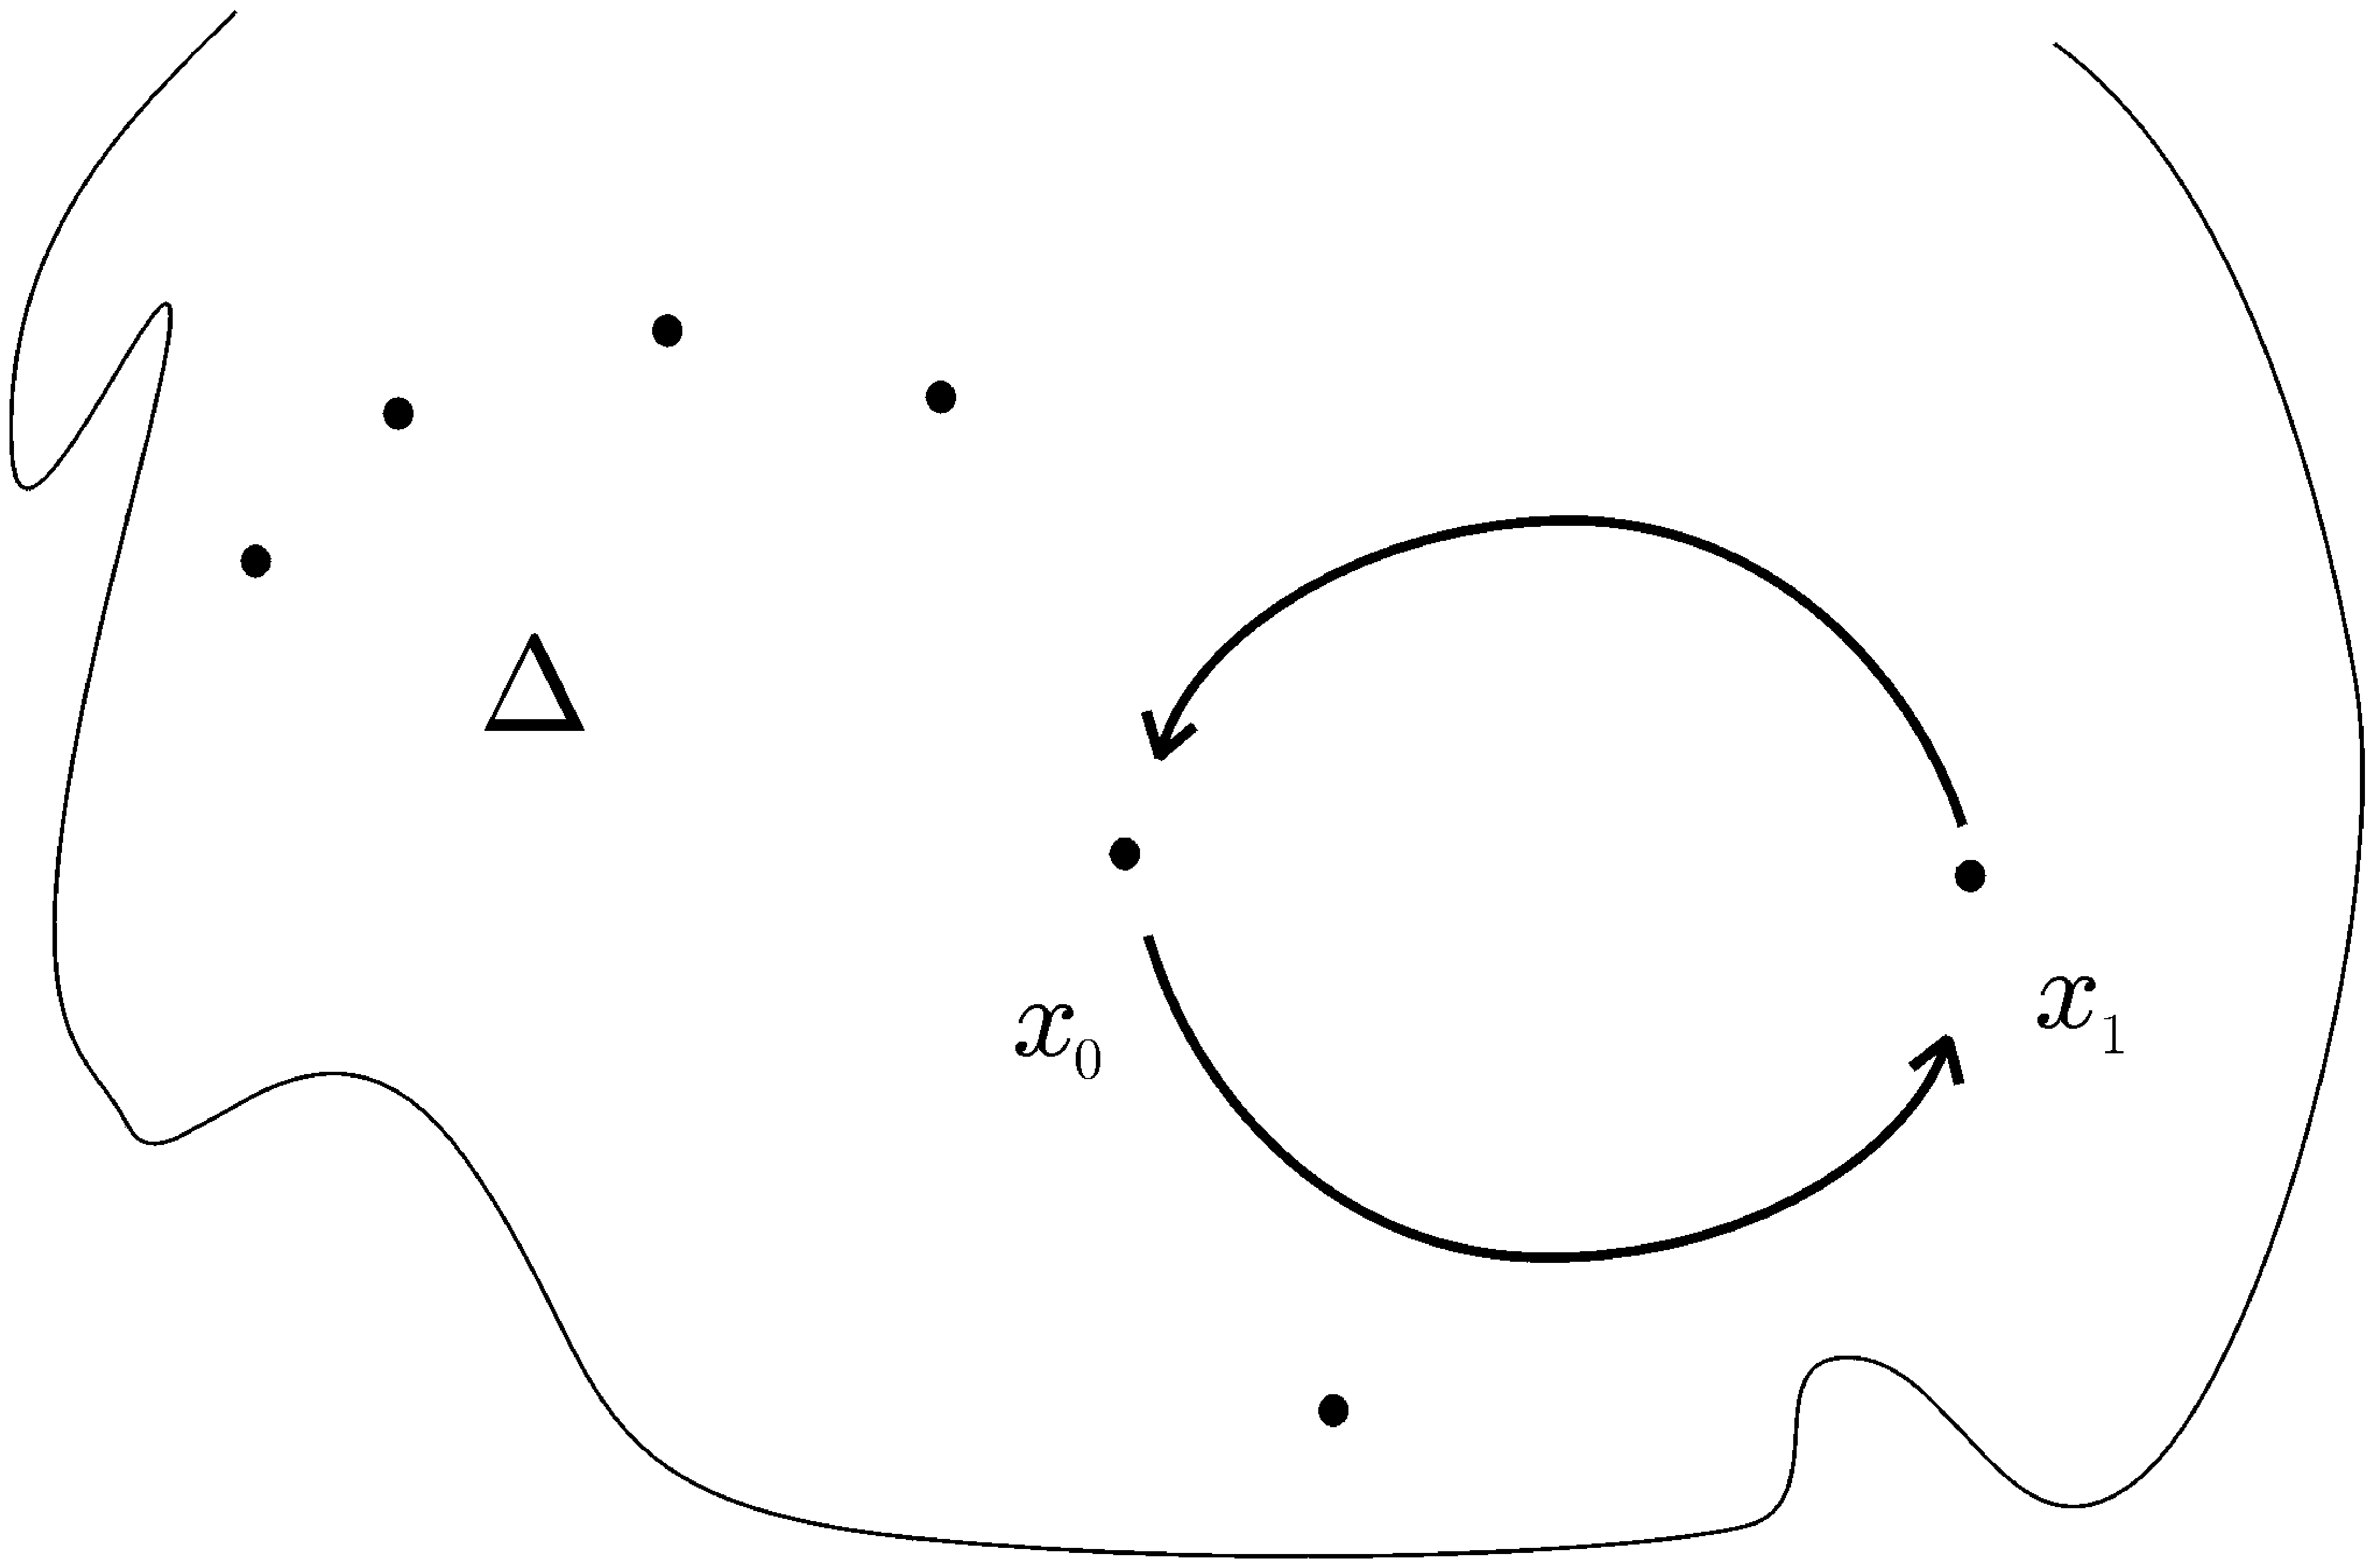
\includegraphics[width=0.5\textwidth]{pict01-5.eps}
\end{center}
 \bigskip
 \refstepcounter{ris}\label{r1-5}

 \centerline{Рис.~\theris}
 \bigskip
\end{figure}




\noindent Если система {$\{f_k\}$~ $(k=0,\ldots,n)$} интерполяционная, то система
уравнений
\[
  \sum\limits^{n}_{k=0}c_k f_k(x_i)=y_i\qquad ({i}=0,\dots ,n),
\]
разрешима для любых {наборов чисел $\{y_k\}$}. {Отсюда следует, что} $\det
(f_k(x_i)) \ne 0$ {для любых $\{x_k\} \subset \Delta$.} По условию функции
$f_k$ непрерывны, следовательно, определитель непрерывен как функция от точек
$\{x_i\}$ в области $\Delta.$ Теперь все точки $x_k$ в $\Delta,$ кроме двух, например
$x_0$ и $x_1$, оставим на месте, а $x_0$ и $x_1$ будем непрерывно переводить друг в
друга {(см. рис.~\ref{r1-5})} {так, что при движении все $n+1$ точки
остаются различными и принадлежат $\Delta$.} Определитель будет непрерывно меняться,
{оставаясь вещественным,} и переменит знак (поменяются местами две строки
определителя). Следовательно, { при каком-то} {промежуточном наборе точек он
обращался в нуль. Это противоречие доказывает } {теорему. }
\end{proof}

\begin{Remark}
Непрерывные действительные интерполяционные
системы не существуют не только на множествах с непустой
внутренностью, но даже на континууме
с точкой ветвления.
\end{Remark}
Действительно, поменяем точки $x_0$ и $x_1$ {местами, перемещая их непрерывно,} как
показано на рис.~\ref{r1-6}, знак определителя изменится, следовательно, он обращался в
нуль, чего  не {должно} быть для непрерывных интерполяционных систем.

%%%%%%%%%%%%%%%%%%%%%%%%%%%%%%%%%%%%%%%%%%%%%%%%%%%%%%
 \bigskip
\begin{figure}[h]
\begin{center}
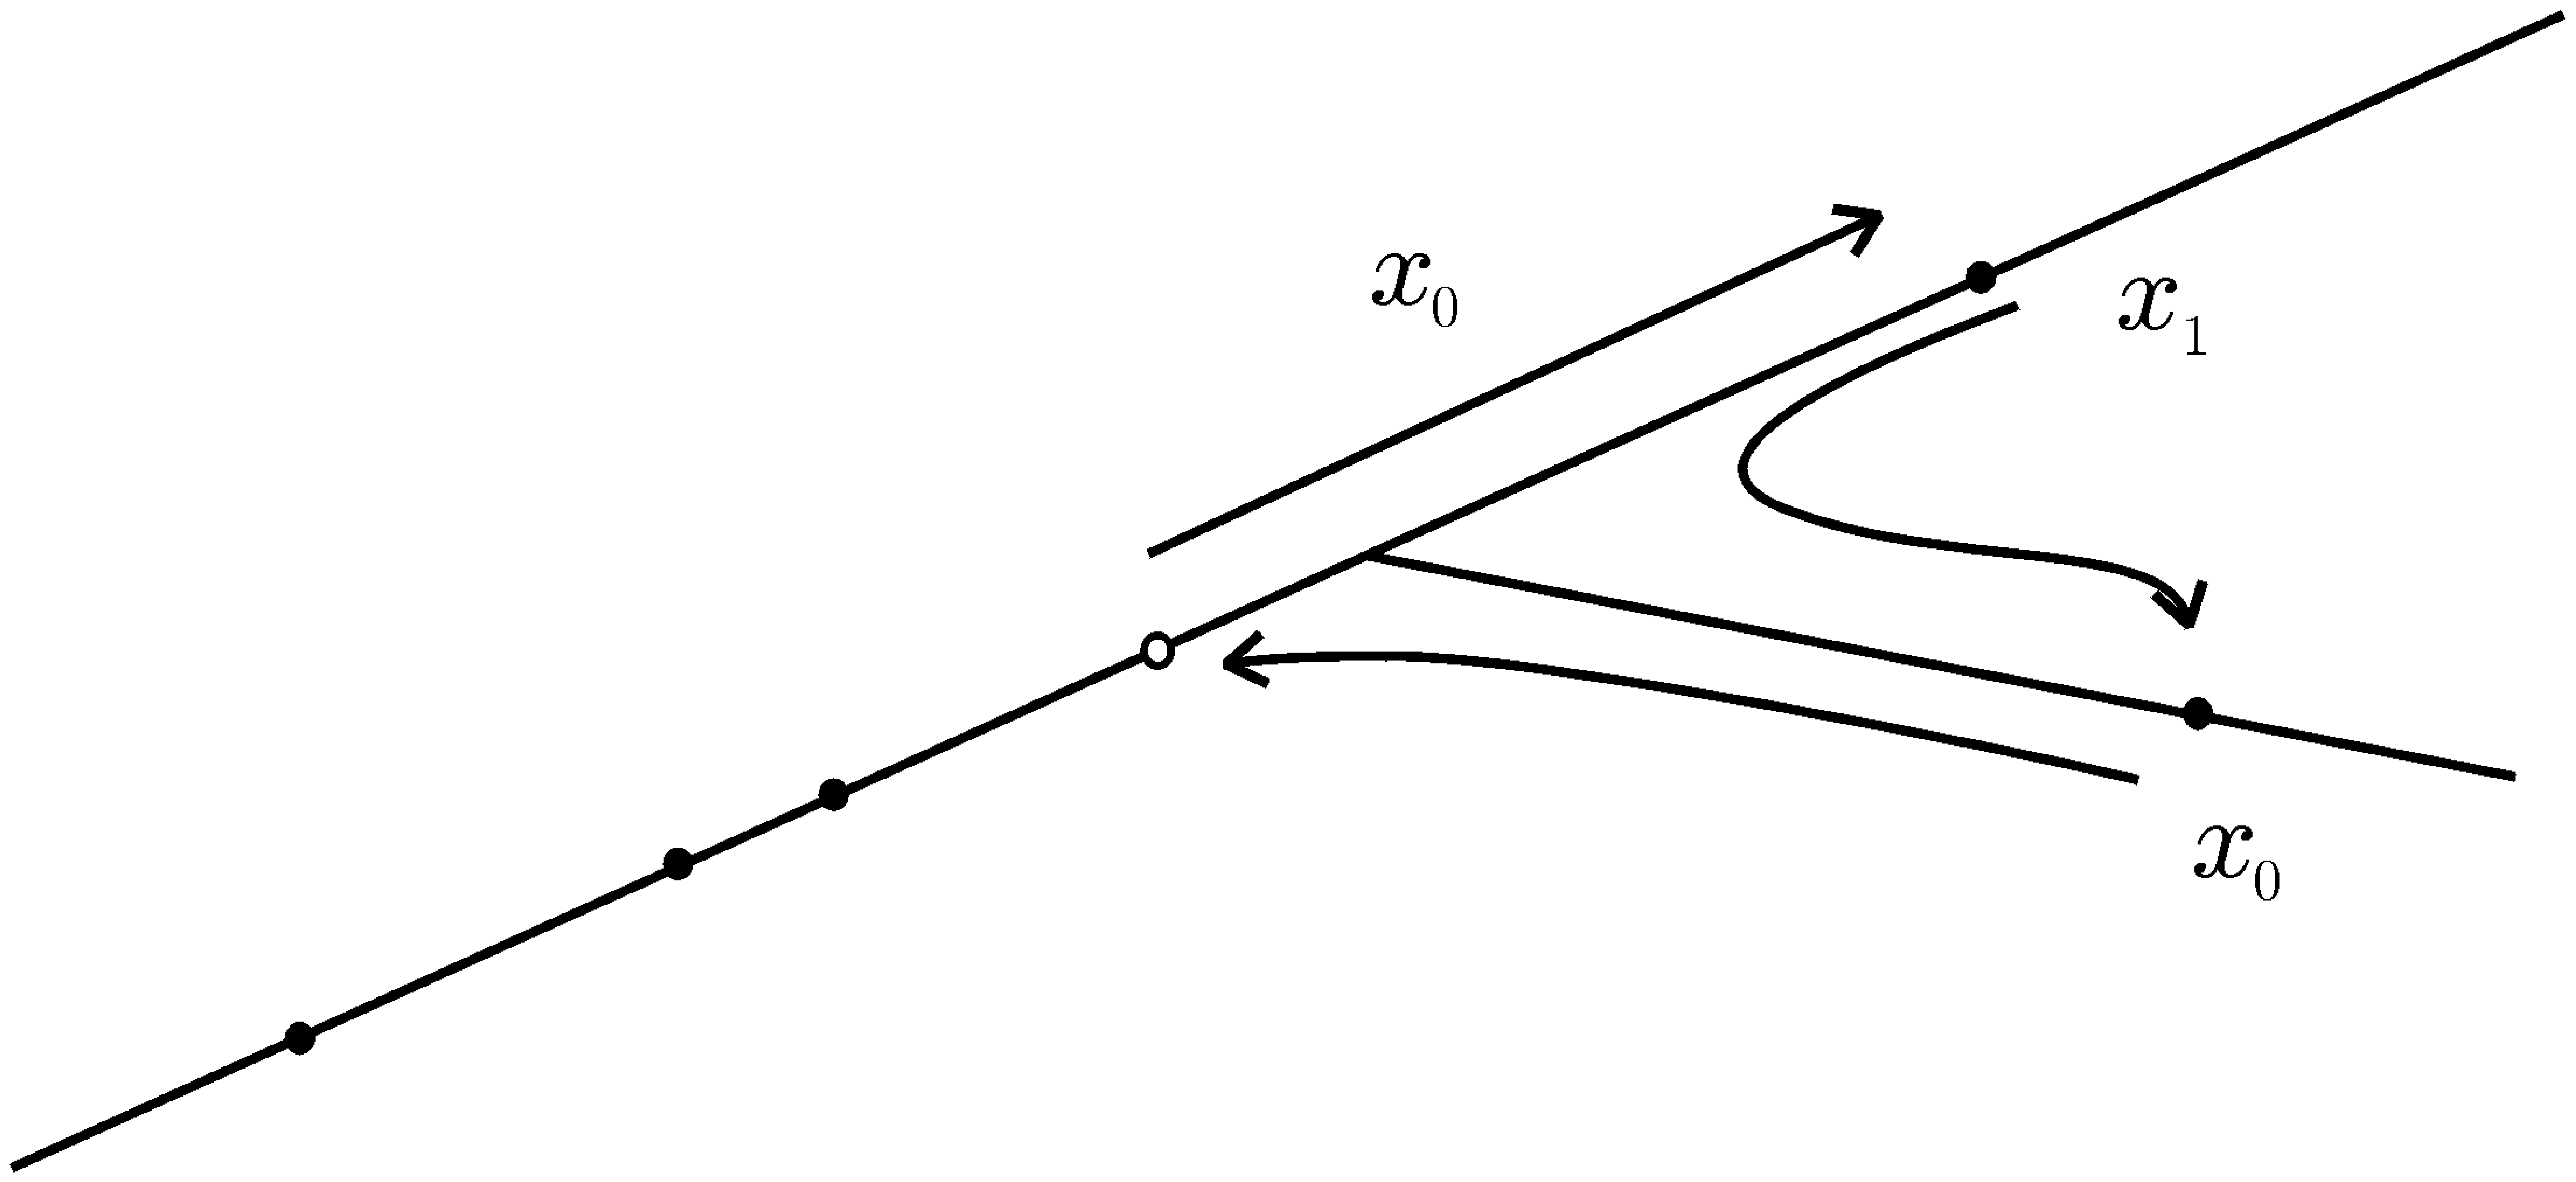
\includegraphics[width=0.5\textwidth]{pict01-6.eps}
\end{center}
 \bigskip
 \refstepcounter{ris}\label{r1-6}

 \centerline{Рис.~\theris}
 \bigskip
\end{figure}


%%%%%%%%%%%%%%%%%%%%%%%%%%%%%%%%%%%%%%%%%%%%%%%%%%%%%%%%%%
%\noindent \hskip3.0cm {рис. 6}
%\bigskip

\noindent
Так что классическая задача интерполяции ограничена
рассмотрением ее на отрезке.

\begin{task}
При чем здесь отрезок? Пусть {$f_k(x) \in \bR^m$}\  $\forall\ x \in K \subset
\bR^M$\ {$(k=0,1,\ldots,n).$} На каких множествах $K$ существуют
непрерывные интерполяционные системы, а для каких не существуют?
\end{task}

При $m \ge 2$ окончательного ответа на эти вопросы нет. Известно (теорема
Мерхьюбера), что при $m=1$ и $n \ge 1$ компактное множество $K$ должно быть гомеоморфно
части
{окружности или всей окружности.
В последнем случае $n$ должно быть четным, т.\,е.} {число базисных функций -- нечетным.
}
